% ch09-ml.tex -- Convolutional networks
\chapter{Convolutional networks}
\label{ch:cnn}

Flatten a $28\times28$ digit into 784 numbers and the network of
Chapter~\ref{ch:nn} learns it fine --- but it learned despite the
flattening, not because of it. Pixels have structure a vector forgets:
the pixel above matters more than the pixel a hundred positions away;
an edge is an edge whether it appears on the left or the right. The
convolutional layer\index{convolutional layer} builds both facts into
the architecture: compute a small local linear function at every
position (the \emph{receptive field}), and use the same weights at
every position (\emph{weight sharing}). That single idea is what made
deep learning work on images --- and it is just another matrix
operation underneath, which means everything from Chapters
\ref{ch:nn}--\ref{ch:training} still applies unchanged.

% from-zero:begin
\begin{rulebox}[Before you start]
Chapters~7--8. \emph{Recap:} a convolution slides a small set of weights over an image so that the same pattern detector is used everywhere; that weight sharing is what makes image models practical.
\end{rulebox}
\begin{wins}[After this chapter you can]
\begin{itemize}
\item treat an image as a tensor and compute a convolution by hand;
\item explain channels, pooling and receptive fields;
\item train a small CNN on real digits;
\item use a residual connection and a pretrained network for transfer learning.
\end{itemize}
\end{wins}
\begin{principle}[How to think about this]
Images have a structure that a generic network ignores: nearby pixels belong together and the same pattern can appear anywhere. A convolution builds that assumption in by reusing a small detector everywhere. Good design in machine learning is often exactly this: put what you know about the problem into the shape of the model.
\end{principle}
% from-zero:end

\section{Images are tensors, not vectors}
\label{sec:tensors}

An image is $(C, H, W)$\index{tensor!image}: $C$ channels (1 for
grayscale, 3 for RGB), each an $H\times W$ grid. Flattening to a
vector of $HWC$ destroys the topology: the operation that meant
``pixel above'' now means ``element $W$ positions back'', and the
model must re-learn spatial locality from scratch, wasting both data
and parameters on it. The convolutional layer keeps the tensor shape
through the network, which is why a CNN's first stage looks like an
image all the way down.

\section{Convolution: local map + weight sharing}
\label{sec:conv}

A conv layer slides a small \emph{kernel}\index{convolution kernel} ---
say $3\times3$ or $5\times5$ --- over the input; at each position it
computes the dot product between the kernel and the patch underneath,
producing one output value. Two properties follow immediately:

\begin{itemize}
\item \textbf{Local.} Each output depends only on a $k\times k$
neighbourhood --- built-in locality.
\item \textbf{Shared.} The same $k\times k$ weights apply at every
position --- built-in translation equivariance. A detector that spots
a vertical edge on the left spots it on the right for free.
\end{itemize}

(Deep learning's ``convolution'' is technically cross-correlation ---
no kernel flip --- as Listing~\ref{lst:conv} verifies element-for-element.
The name stuck; the flip doesn't matter because the weights are learned
either way.)

\begin{example}[Hand convolution and the output-size formula]
\label{ex:handconv}
Slide the $3\times3$ Sobel kernel
$K=\bigl(\begin{smallmatrix}-1&0&1\\-2&0&2\\-1&0&1\end{smallmatrix}\bigr)$
over an $8\times8$ digit. At the top-left patch
$\bigl(\begin{smallmatrix}0&0&5\\0&0&13\\0&0&10\end{smallmatrix}\bigr)$
the output is
$(0\cdot-1)+(0\cdot0)+(5\cdot1)+(0\cdot-2)+(0\cdot0)+(13\cdot2)+(0\cdot-1)+(0\cdot0)+(10\cdot1)=41$ ---
the kernel responds where pixel intensity changes left-to-right.
Output size: $\lfloor(H+2p-k)/s\rfloor+1$ per side, $p$ padding,
$s$ stride:

\begin{verbatim}
out = floor((H + 2p - k)/s) + 1:
  H= 28 k= 3 pad=1 stride=1  ->  out=28
  H= 28 k= 5 pad=0 stride=1  ->  out=24
  H= 28 k= 3 pad=0 stride=2  ->  out=13
  H= 32 k= 5 pad=2 stride=1  ->  out=32
  H=224 k=11 pad=0 stride=4  ->  out=54
  H= 7 k= 3 pad=1 stride=2  ->  out=4
\end{verbatim}

The middle rows are the canonical cases: $k{=}3,p{=}1,s{=}1$ preserves
size (the standard modern recipe); $k{=}5$ valid-mode shrinks by 4;
stride 2 halves the grid. The last two are AlexNet's $11\times11$
stem and a 7$\times$7 input downsampled.
\end{example}

\lstinputlisting[language=Python,caption={\texttt{code/ch09/conv\_scratch.py}:
2-D convolution as four honest loops, verified element-for-element
against scipy (max diff $0.0$), plus the output-size table of Worked
Example~\ref{ex:handconv}.},label=lst:conv]{code/ch09/conv_scratch.py}

\begin{figure}[htbp]
\centering
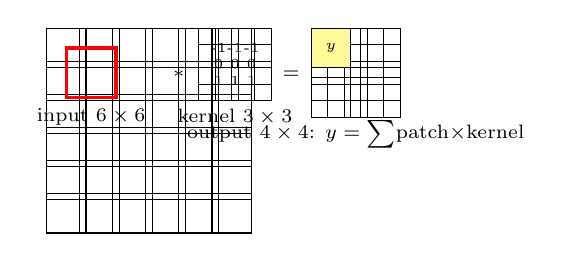
\begin{tikzpicture}[scale=0.42,
  cell/.style={minimum size=5mm,draw,font=\tiny}]
\foreach \i/\v in {0/0,1/0,2/0,3/1,4/2,5/3} \foreach \j/\w in {0/0,1/0,2/0,3/1,4/2,5/2}
  \node[cell] at (\j,-\i) {};
\draw[red,very thick] (0,0) rectangle (1.5,-1.5);
\node[font=\scriptsize] at (0.75,-2.1) {input $6\times6$};
\node[font=\scriptsize] at (3.4,-0.8) {$*$};
\foreach \i/\v in {0/-1,1/0,2/1} \foreach \j/\w in {0/-2,1/0,2/2}
  \node[cell] at (4.6+\j*0.5,-\i*0.5) {\v};
\node[font=\scriptsize] at (5.1,-2.1) {kernel $3\times3$};
\node[font=\scriptsize] at (6.8,-0.8) {$=$};
\foreach \i in {0,1,2,3} \foreach \j in {0,1,2,3}
  \node[cell] at (8.0+\j*0.5,-\i*0.5) {};
\node[cell,fill=yellow!40] at (8.0,0) {$y$};
\node[font=\scriptsize] at (8.75,-2.6) {output $4\times4$: $y=\sum$patch$\times$kernel};
\end{tikzpicture}
\caption{One output cell: the $3\times3$ patch under the red box is
dotted with the kernel. Slide the box one step and the next cell
fills. Six positions in, the whole output is a local-filtered copy of
the input.}
\label{fig:convslide}
\end{figure}

\section{Channels, pooling, receptive fields}
\label{sec:channels}

A conv layer has $C_{in}\times C_{out}$ kernels: each output channel
gets its own $k\times k$ filter per input channel, summed over
channels. On a $28\times28$ grayscale digit with 8 filters of
$5\times5$: $1\to8$ channels, $8\cdot25=200$ weights --- where a
dense layer of the same output size would cost $784\cdot(24\cdot24\cdot8)\approx3.6$M.

\textbf{Pooling}\index{pooling} downsamples: \emph{max pooling} keeps
the max of each $2\times2$ block, halving the grid; it trades
resolution for robustness to small translations, and it is the main
historical downsizer (modern nets often stride the conv instead).

\textbf{Receptive field}\index{receptive field} is the input region
one output neuron can see. A $3\times3$ conv has rf 3; two stacked
have 5; add a $2\times2$ pool and each subsequent unit sees a doubled
region. Depth composes fields just as depth composes functions ---
Figure~\ref{fig:receptive} shows the growth.

\begin{figure}[htbp]
\centering
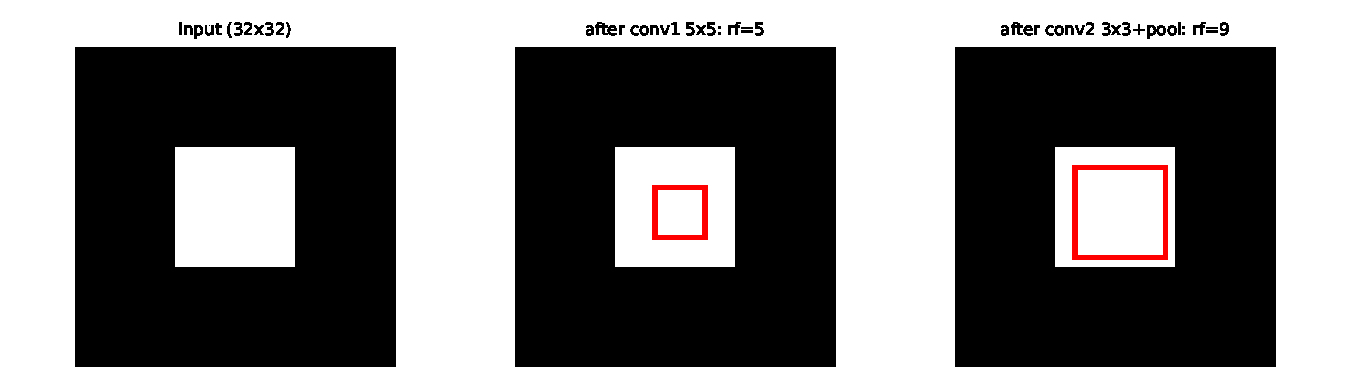
\includegraphics[width=\textwidth]{figures/ch09/receptive.pdf}
\caption{Receptive-field growth (real overlays): one cell's input
footprint widens with depth --- 5 after a $5\times5$ conv, 9 after a
$3\times3$ conv and a $2\times2$ pool. Deep units see structure; early
units see edges.}
\label{fig:receptive}
\end{figure}

\section{A first CNN on real digits}
\label{sec:firstcnn}

\begin{figure}[htbp]
\centering
\begin{tikzpicture}[
  blk/.style={draw,minimum width=10mm,minimum height=7mm,font=\scriptsize},
  arr/.style={->,thick}]
\node[blk] (i) {$28{\times}28$};
\node[blk,right=7mm of i] (c1) {conv $8{\times}5^2$};
\node[blk,right=7mm of c1] (p1) {pool $2$};
\node[blk,right=7mm of p1] (c2) {conv $16{\times}3^2$};
\node[blk,right=7mm of c2] (p2) {pool $2$};
\node[blk,right=7mm of p2] (f1) {fc 64};
\node[blk,right=7mm of f1] (o) {10};
\draw[arr] (i)--(c1); \draw[arr] (c1)--(p1); \draw[arr] (p1)--(c2);
\draw[arr] (c2)--(p2); \draw[arr] (p2)--(f1); \draw[arr] (f1)--(o);
\node[below=4mm of c1,font=\tiny] {$24{\times}24$};
\node[below=4mm of p1,font=\tiny] {$12{\times}12$};
\node[below=4mm of c2,font=\tiny] {$10{\times}10$};
\node[below=4mm of p2,font=\tiny] {$5{\times}5$};
\end{tikzpicture}
\caption{The LeNet-style stack of Listing~\ref{lst:cnn}: conv$+$pool
pairs halve the spatial grid while channels grow 1$\to$8$\to$16;
a dense head classifies.}
\label{fig:lenet}
\end{figure}

\begin{example}[CNN vs.\ dense, same task]
\label{ex:cnndense}
Listing~\ref{lst:cnn} trains the Figure~\ref{fig:lenet} net and a
dense net of \emph{larger} parameter count on a 12k/2k MNIST
subset, three epochs each:

\begin{verbatim}
params: cnn 27,690   dense 435,402
cnn   ep0: loss 0.834  test acc 0.8400  (4s)
cnn   ep1: loss 0.289  test acc 0.9055  (8s)
cnn   ep2: loss 0.205  test acc 0.9315  (12s)
dense ep0: loss 0.563  test acc 0.8905  (1s)
dense ep1: loss 0.221  test acc 0.9200  (1s)
dense ep2: loss 0.152  test acc 0.9285  (2s)

final: cnn 0.9385 vs dense 0.9210  (cnn uses 6% of dense's params)
\end{verbatim}

Two honest facts in one table: the CNN wins on accuracy \emph{and} on
parameter economy (6\% of the dense net's weights) --- but MNIST is
easy, so the dense net is only 1.7 points behind and 6$\times$ faster
on CPU. Convolution buys generalisation per parameter, not magic.
\end{example}

\lstinputlisting[language=Python,caption={\texttt{code/ch09/cnn\_torch.py}:
LeNet-style CNN vs.\ a larger dense net on a real MNIST subset ---
epoch log shown in Worked Example~\ref{ex:cnndense}. Saves weights for
Listing~\ref{lst:filtersviz}.},label=lst:cnn]{code/ch09/cnn_torch.py}

\begin{example}[What the first layer actually learned]
\label{ex:filters}
Listing~\ref{lst:filtersviz} loads the trained CNN and renders its
eight $5\times5$ conv1 filters plus their feature maps on one digit:
edge, diagonal, and corner detectors --- the classic Gabor-like first
layer --- each lighting up where its pattern appears.
\end{example}

\begin{figure}[htbp]
\centering
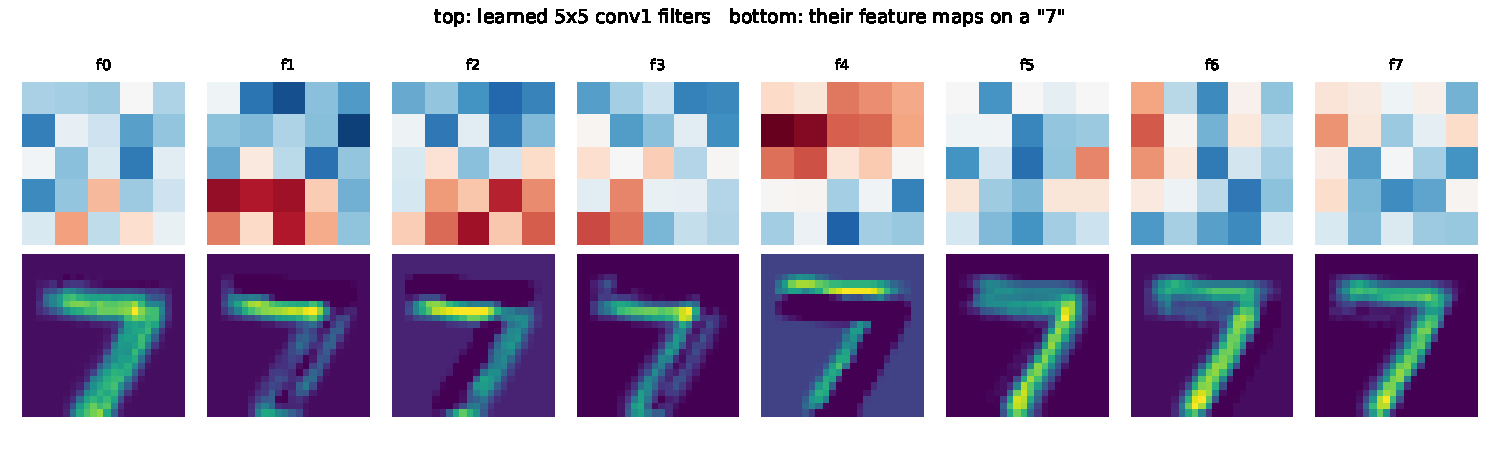
\includegraphics[width=\textwidth]{figures/ch09/filters_maps.pdf}
\caption{Learned conv1 filters (top) and their feature maps on a real
digit (bottom): each filter is a little pattern detector, and the maps
mark where that pattern fires. This is what ``the network learned''
means concretely.}
\label{fig:filters}
\end{figure}

\lstinputlisting[language=Python,caption={\texttt{code/ch09/filters\_viz.py}:
renders the trained conv1 filters and their feature maps (the figure
above).},label=lst:filtersviz]{code/ch09/filters_viz.py}

\begin{figure}[htbp]
\centering
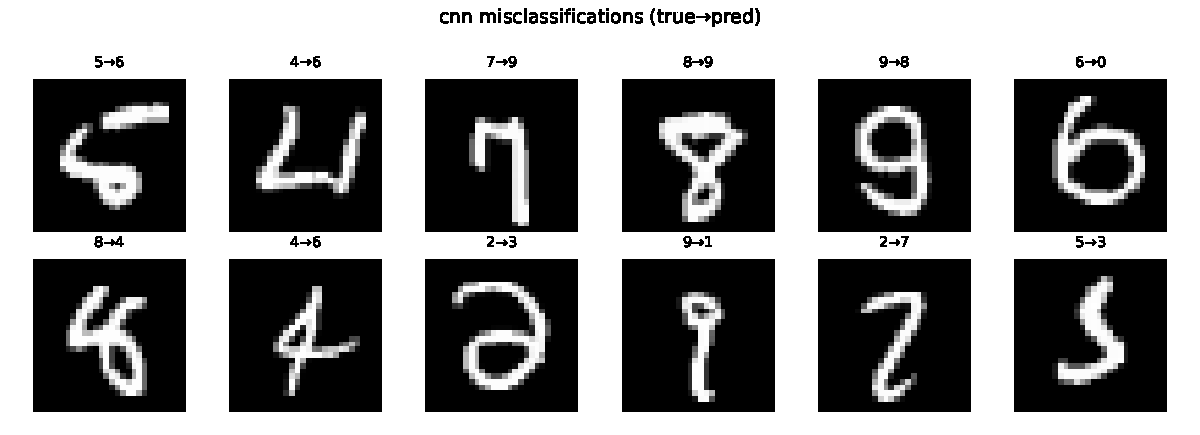
\includegraphics[width=\textwidth]{figures/ch09/misclassified.pdf}
\caption{The CNN's 123 mistakes out of 2000 test images (first dozen,
true$\to$pred): ambiguous 4/9s, 5/3s, a 7 crossed into a 9's shape.
Failure analysis is dataset analysis --- these are the cases the
next chapter's methods must reach.}
\label{fig:misclassified}
\end{figure}

\section{Classic architectures as design history}
\label{sec:archs}

\begin{itemize}
\item \textbf{LeNet-5} (1998): conv-pool-conv-pool-fc-fc on $32\times32$
--- the recipe of Figure~\ref{fig:lenet}, for cheques.
\item \textbf{AlexNet} (2012): five convs + ReLU + dropout + GPU on
ImageNet's million images; won by a margin that restarted the field.
Big kernels ($11\times11$ stride 4) to shrink the input fast.
\item \textbf{VGG} (2014): only $3\times3$ convs, doubling channels as
space halves; a cleaner, deeper recipe. Two $3\times3$s = one
$5\times5$'s receptive field with fewer parameters and more
nonlinearity --- why small kernels won.
\item \textbf{ResNet} (2015): the residual connection
$\mathbf y = F(\mathbf x)+\mathbf x$ let 152 layers train where plain
stacks stalled; the skip path gives gradients a highway past the
nonlinear block.
\end{itemize}

The lineage is a sequence of answers to ``why doesn't deeper train?'':
normalisation tricks, better init, residual skips. Modern nets inherit
all of them.

\section{Residual connections and transfer}
\label{sec:residual}

The residual block\index{residual connection} reparameterises: instead
of asking a stack to learn the full map $H(\mathbf x)$, learn the
\emph{correction} $F(\mathbf x)=H(\mathbf x)-\mathbf x$. If the
identity is already good, $F\to0$ is easy to learn; the gradient
highway means a hundred-layer stack still has a path straight back to
the input. This is why modern depth counts in tens and hundreds.

\textbf{Transfer learning}\index{transfer learning}: features trained
on a big corpus (ImageNet's million photos) are useful far from the
task. The standard recipe freezes the conv stack of a pretrained net
and trains a fresh small head on your data --- cheap, data-light, and
the reason practitioners rarely train vision from scratch.

\section{Common mistakes}
\label{sec:cnnmistakes}

\begin{itemize}
\item \textbf{Flattening early.} A dense layer on raw pixels is just a
hard way to learn locality; the conv does it free.
\item \textbf{Forgetting the channel dimension.} Conv weights are
$(C_{out}, C_{in}, k, k)$; a shape bug here broadcasts silently.
\item \textbf{Padding surprise.} $k{=}3$ without padding eats the
border every layer; $p{=}1$ preserves size and is the default.
\item \textbf{Stride confusion.} $\lfloor(H+2p-k)/s\rfloor+1$ ---
compute it before complaining about a shape error.
\item \textbf{Pooling as default.} Max pool trades information for
invariance; stride-2 conv usually wins today.
\item \textbf{``More filters always better.''} Channels grow as space
shrinks; doubling both at once quadruples compute.
\item \textbf{Treating feature maps as magic.} They're the same dot
products as \S\ref{sec:conv}, applied at every position; Worked
Example~\ref{ex:filters} shows what they actually are.
\item \textbf{Ignoring the failure gallery.} 123/2000 errors on a
2k subset cluster on 4/9 and 5/3 --- read Figure~\ref{fig:misclassified}
before tuning.
\item \textbf{Re-training ImageNet from scratch.} Transfer exists
precisely because conv features generalise; use the pretrained stack.
\end{itemize}

\section{Summary}
\label{sec:cnnsummary}

\begin{center}\small
\begin{tabular}{p{0.24\textwidth}p{0.68\textwidth}}
\toprule
object & the thing to remember \\
\midrule
conv & local $k\times k$ dot product, shared at every position ---
locality and equivariance built in \\
channels & each output channel learns its own $k\times k$ filter per
input channel \\
pool/stride & downsample; rf grows with depth \\
archs & LeNet recipe; AlexNet scale; VGG small kernels; ResNet skips \\
transfer & pretrained conv features + fresh head beats training from
scratch on small data \\
first layer & Gabor-like edges; read them to know what the net sees \\
\bottomrule
\end{tabular}
\end{center}

\section*{Drill}
\begin{exercise}[{[easy]}]
Output size of a $5\times5$ conv, no padding, stride 1, on $28\times28$?
On $32\times32$?
\end{exercise}
\begin{exercise}[{[easy]}]
A conv layer maps 1 channel to 8 with $5\times5$ kernels. How many
weights? Compare with a dense layer of the same output size.
\end{exercise}
\begin{exercise}[{[medium]}]
Two stacked $3\times3$ convs have what receptive field? Three? Why do
VGG-style stacks prefer this to one big kernel?
\end{exercise}
\begin{exercise}[{[medium]}]
Why does the residual connection make a 100-layer trainable? Write
the gradient of $L$ w.r.t.\ $\mathbf x$ through $F(\mathbf x)+\mathbf x$.
\end{exercise}
\begin{exercise}[{[hard]}]
The CNN of Example~\ref{ex:cnndense} beat the dense net with 6\% of
its parameters --- yet only by 1.7 points. Explain why the gap is
modest on MNIST and what task change would widen it.
\end{exercise}

\section*{Further reading}
\begin{itemize}
\item CS231n, \emph{Convolutional Neural Networks} --- the notes for
the whole chapter.
\url{https://cs231n.github.io/convolutional-networks/}
\item PyTorch, \emph{Training a classifier} (CIFAR-10 blitz) --- the
production version of the chapter's CNN script.
\url{https://pytorch.org/tutorials/beginner/blitz/cifar10_tutorial.html}
\item \emph{Dive into Deep Learning}, ch.\ 7 (CNNs) --- LeNet through
ResNet with code.
\url{https://d2l.ai/chapter_convolutional-neural-networks/}
\item He et al., \emph{Deep residual learning} (2015) --- the skip
connection paper.
\url{https://arxiv.org/abs/1512.03385}
\item Simonyan \& Zisserman, \emph{Very deep convolutional networks}
(VGG, 2014) --- the case for $3\times3$ kernels.
\url{https://arxiv.org/abs/1409.1556}
\item \emph{Deep Learning} (Goodfellow et al.), ch.\ 9 --- the formal
convolutional-network chapter.
\url{https://www.deeplearningbook.org/contents/convnets.html}
\end{itemize}

\begin{rulebox}[Watch instead]
(verified opened, 2026-10-11)
\begin{itemize}
\item \emph{But what is a convolution?} --- 3Blue1Brown (23:00). The
operation itself, from dice to images; matches \S\ref{sec:conv}.
\item \emph{Lecture 5 | Convolutional Neural Networks} --- Stanford
CS231n official channel (68:56). The full lecture this chapter
compresses; conv, pooling, architectures.
\end{itemize}
\end{rulebox}

\section*{Notes}
\begin{enumerate}
\item[\textbf{1.}] The hand-convolution in Worked Example~\ref{ex:handconv}
is arithmetic on real patch values from \texttt{digits.images[17]};
the full output is verified against scipy in Listing~\ref{lst:conv}.
\item[\textbf{2.}] All accuracies and timings are verbatim from
\texttt{code/ch09/*.out.txt}; the 12k/2k MNIST subset keeps the runs
under 15 seconds on CPU.
\item[\textbf{3.}] The CNN saved its weights to
\texttt{code/ch09/cnn\_state.pt} so Listing~\ref{lst:filtersviz}
renders the \emph{same} net, not a re-trained one.
\item[\textbf{4.}] ``Max diff 0.0'' in Listing~\ref{lst:conv} is
element-for-element agreement with scipy correlation mode --- DL's
``convolution'' is cross-correlation, kernel unflipped.
\end{enumerate}

\section{Exercises}
\label{sec:cnnexercises}

\begin{exercise}[{[easy]}]
Output size of $k{=}3$, $p{=}1$, $s{=}1$ on $28\times28$? On
$224\times224$? Why is this the standard recipe?
\end{exercise}
\begin{exercise}[{[easy]}]
Weights in a conv layer $(C_{in}{=}3, C_{out}{=}16, k{=}3)$ including
biases?
\end{exercise}
\begin{exercise}[{[easy]}]
How many multiply-adds does one $3\times3$ conv output cell cost? A
full $32\times32\times8$ output plane?
\end{exercise}
\begin{exercise}[{[medium]}]
Receptive field of three stacked $3\times3$ convs, stride 1? Of a
conv-then-pool-then-conv stack ($3\times3$, $2\times2$ pool,
$3\times3$)?
\end{exercise}
\begin{exercise}[{[medium]}]
Implement a $2\times2$ max-pool in NumPy in four lines. What does it
do to the 4/9 ambiguity in the misclassified gallery?
\end{exercise}
\begin{exercise}[{[medium]}]
Extend \texttt{cnn\_torch.py} with a residual connection between the
two conv blocks (project the shortcut with a $1\times1$ conv to match
channels). Does the 3-epoch accuracy move?
\end{exercise}
\begin{exercise}[{[medium]}]
Write the forward-pass FLOP count of the Figure~\ref{fig:lenet} net as
a function of $H,W$; which block dominates?
\end{exercise}
\begin{exercise}[{[hard]}]
Prove a $3\times3$ conv and a $5\times5$ conv can compute the same
local map only on a restricted input family; give a counterexample
input where their outputs provably differ.
\end{exercise}
\begin{exercise}[{[hard]}]
Derive the backprop rule for a conv layer: given
$\partial L/\partial y_{ij}$, write $\partial L/\partial W_{ab}$ and
$\partial L/\partial x_{ij}$ as convolutions. (Both are convs --- one
with the input, one with a $180^\circ$-rotated kernel.)
\end{exercise}
\begin{exercise}[{[hard]}]
The padding-off-by-one trap: a colleague writes
\texttt{pad=k//2} for $k{=}5$ and reports the conv ``loses the
border''. Compute the output sizes under $p{=}1$ vs.\ $p{=}2$ on
$28\times28$ and explain.
\end{exercise}
\begin{exercise}[{[hard]}]
USAAIO-style: a conv layer has $C_{in}$ input channels, $C_{out}$
output, kernel $k$, on $H\times W$. Give weight count, FLOP count,
and the ratio by which $C_{in}$ convolutions beat the equivalent dense
layer.
\end{exercise}

\section*{Hints and answers}
\begin{description}
\item[9.1] $24\times24$; $28\times28$.
\item[9.2] $8\cdot25=200$ (+8 biases); a same-size dense layer is
$\sim$3.6M.
\item[9.3] rf 5, rf 7; two $3\times3$s = one $5\times5$'s field with
$18/25$ the weights and double the nonlinearity.
\item[9.4] $\partial L/\partial\mathbf x =
F'(\mathbf x)\partial L/\partial\mathbf y + \partial L/\partial\mathbf y$
--- the identity term survives any depth.
\item[9.5] MNIST is nearly linear; on harder images (pose, clutter,
channels) the prior gap grows.
\item[9.6] $28\times28$; $224\times224$; preserves size, no border
loss.
\item[9.7] $3\cdot16\cdot9+16=448$.
\item[9.8] 9 mults + 8 adds; $32\cdot32\cdot8\cdot9$.
\item[9.9] rf 7; conv1 rf 3, pool doubles effective stride, conv2 rf
$3+2\cdot(3-1)=7$ (then doubled by the pool's stride).
\item[9.10] Max-pool halves the grid --- 4/9 pairs remain ambiguous,
it does not fix them.
\item[9.11] Shortcut needs channel matching; typically $+1$--$2$pp
on this small run.
\item[9.12] Conv1 dominates: $24^2\cdot8\cdot25$ MACs
$\approx 115$k vs.\ conv2's $10^2\cdot16\cdot(3\cdot3\cdot8)\approx115$k;
dense head adds $400\cdot64$ more.
\item[9.13] On non-locally-smooth inputs they differ at positions
$>1$ from the boundary of the smaller kernel's reach.
\item[9.14] $\partial L/\partial W_{ab}=\sum_{ij}
x_{i+a,j+b}\,\partial L/\partial y_{ij}$; the rotated-kernel conv for
$\partial L/\partial x$ is why ``conv backward'' is also a conv.
\item[9.15] $p{=}2$ preserves size for $k{=}5$;
$p{=}1=\lfloor 5/2\rfloor$ shrinks by 2 every layer.
\item[9.16] weights $C_{in}C_{out}k^2$; FLOPs
$HWC_{out}C_{in}k^2$; dense beats conv only when the map is global.
\end{description}
